%% ----------------------------------------------------------------
%% PACKAGES
%% ----------------------------------------------------------------
\documentclass[titlepage, 12pt]{article}
\usepackage[table, xcdraw, dvipsnames]{xcolor}
\usepackage[utf8]{inputenc}
\usepackage[spanish, es-tabla]{babel}
\usepackage{amsmath}
\usepackage{biblatex}
\usepackage{booktabs}
\usepackage[RPvoltages]{circuitikz}
\usepackage{csquotes}
\usepackage{enumitem}
\usepackage{fancyhdr}
\usepackage{float}
\usepackage{geometry}
\usepackage{graphicx}
\usepackage[hidelinks]{hyperref}
\usepackage{lastpage}
\usepackage{pdflscape}
\usepackage{parskip}
\usepackage{pdfpages}
\usepackage{siunitx}
\usepackage{subcaption}
\usepackage{subfiles}
\usepackage{tabularx}
\usepackage{tikz}
\usepackage{xfrac}


%% ----------------------------------------------------------------
%% SETTINGS
%% ----------------------------------------------------------------
\decimalpoint
\geometry{
  a4paper,
  total={170mm,247mm},   %210x297mm
  left=20mm,
  top=20mm,
}
\newcommand{\fecha}{16/08/2021} % #FIXME
\newcommand{\version}{1.0}

\usetikzlibrary{shapes, arrows, babel}
\tikzstyle{block} = [draw, fill=gray!5, rectangle, minimum height=3em, minimum width=6em]
\tikzstyle{sum} = [draw, fill=gray!10, circle, node distance=2cm]
\tikzstyle{input} = [coordinate]
\tikzstyle{output} = [coordinate]
\tikzstyle{pinstyle} = [pin edge={to-,thin,black}]
\tikzstyle{branch} = [circle,inner sep=0pt,minimum size=1mm,fill=black,draw=black]

\def\normalcoord(#1){coordinate(#1)}
\def\showcoord(#1){node[circle, red, draw, inner sep=1pt, pin={[red, overlay, inner sep=0.5pt, font=\tiny, pin distance=0.1cm, pin edge={red, overlay}]45:#1}](#1){}}
\let\coord=\normalcoord

\addbibresource{../informe/bibliography.bib}


%% ----------------------------------------------------------------
%% HEADER/FOOTER
%% ----------------------------------------------------------------
\pagestyle{fancy}
\fancyhf{}
\lhead{Calibrador y caracterizador de sondas de corriente}
\rhead{Especificación técnica}
\lfoot{Fecha: \fecha}
\cfoot{Versión \version}
\rfoot{Página \thepage \hspace{1pt} de \pageref{LastPage}}

\setlength{\headheight}{30pt}


%% ----------------------------------------------------------------
%% TITLE
%% ----------------------------------------------------------------
\title{Especificación técnica:\\Calibrador y caracterizador de sondas de corriente}
\author{Agustín Aon Sanchez\\
Facultad de Ingeniería\\
Universidad Nacional de Mar del Plata}
\date{Versión \version}


%% ----------------------------------------------------------------
%% BEGIN
%% ----------------------------------------------------------------
\begin{document}
\maketitle


%% ----------------------------------------------------------------
%% DOCUMENT
%% ----------------------------------------------------------------

%% ----------------------------------------------------------------
\section{Ficha del documento}
%% ----------------------------------------------------------------
\begin{table}[!hbtp]
  \centering
  \begin{tabular}{|c|c|c|c|}
  \hline
  \rowcolor[HTML]{C0C0C0}
  Fecha  & Versión  & Descripción     & Autor               \\ \hline
  \fecha & \version & Versión inicial & Agustín Aon Sanchez \\ \hline
  \end{tabular}
\end{table}

\newpage
\tableofcontents
\newpage
\listoffigures
\listoftables
\newpage

%% ----------------------------------------------------------------
\section{Introducción}
%% ----------------------------------------------------------------
Este documento corresponde a la Especificación Técnica para el proyecto final titulado Calibrador y caracterizador de sondas de corriente. Esta especificación se ha estructurado basándose en la información mencionada en el documento Especificación de Requerimientos (ER) versión 3.0 y en el documento Especificación Funcional (EF) versión 1.0. %FIXME

  %% ----------------------------------------------------------------
  \subsection{Propósito del documento}
  %% ----------------------------------------------------------------
  El presente documento tiene como propósito proveer información detallada de cómo funcionará la solución, cuáles serán sus comportamientos deseados y cómo se deberá construir, con base en los requerimientos anteriormente definidos en la ER.

  Esta especificación funciona está dirigida a aquellos encargados del desarrollo de este proyecto. Además, este documento puede servir de soporte a aquellas personas que en un futuro deseen realizar un dispositivo similar.

  %% ----------------------------------------------------------------
  \subsection{Alcance del proyecto}
  %% ----------------------------------------------------------------
  El proyecto abarca la definición de los requerimientos, la implementación de la solución y la presentación final de la misma.

  Los requerimientos fueron planteados junto con el Laboratorio de Instrumentación y Control (LIC) de la Facultad de Ingeniería de la Universidad Nacional de Mar del Plata. Es en este laboratorio donde se realizará la mayor parte de este proyecto, haciendo uso de los recursos disponibles, bajo la guía del director del proyecto.

  La implementación de la solución será también realizada en el LIC.

  %% ----------------------------------------------------------------
  \subsection{Personal involucrado}
  %% ----------------------------------------------------------------
  \begin{table}[!hbtp]
    \centering
    \begin{tabularx}{\textwidth}{| >{\columncolor[HTML]{C0C0C0}}l |X|}
      \hline
      Nombre                  & Agustín Aon Sanchez             \\ \hline
      Rol                     & Desarrollador                   \\ \hline
      Categoría Profesional   & Estudiante                      \\ \hline
      Responsabilidad         & Desarrollo y diseño del sistema \\ \hline
      Información de contacto & agustin.aon.s@gmail.com         \\ \hline
    \end{tabularx}
  \end{table}

  \begin{table}[!hbtp]
    \centering
    \begin{tabularx}{\textwidth}{| >{\columncolor[HTML]{C0C0C0}}l |X|}
      \hline
      Nombre                  & Ignacio Carugati        \\ \hline
      Rol                     & Director                \\ \hline
      Categoría Profesional   & Investigador            \\ \hline
      Responsabilidad         & Supervisar y guiar el desarrollo del proyecto \\ \hline
      Información de contacto & icarugati@fi.mdp.edu.ar \\ \hline
    \end{tabularx}
  \end{table}

  %% ----------------------------------------------------------------
  \subsection{Definiciones, acrónimos y abreviaturas}
  %% ----------------------------------------------------------------
  \begin{table}[H]
    \centering
    \begin{tabular}{|c|l|}
    \hline
      \rowcolor[HTML]{C0C0C0}
      Nombre & \multicolumn{1}{c|}{\cellcolor[HTML]{C0C0C0}Descripción} \\ \hline
      ADC    & Conversor Analógico Digital                              \\ \hline
      API    & Protocolo de interfaz de aplicación                      \\ \hline
      CSV    & Formato de archivos de datos                             \\ \hline
      JPG    & Formato de archivos de imágenes                          \\ \hline
      LIC    & Laboratorio de Instrumentación y Control                 \\ \hline
      PC     & Computadora Personal                                     \\ \hline
      PDF    & Formato de archivos de documentos                        \\ \hline
      PNG    & Formato de archivos de imágenes                          \\ \hline
      RC     & Controlador repetitivo                                   \\ \hline
      RF     & Requerimiento Funcional                                  \\ \hline
      RNF    & Requerimiento No Funcional                               \\ \hline
    \end{tabular}
  \end{table}

  %% ----------------------------------------------------------------
  \subsection{Referencias}
  %% ----------------------------------------------------------------
  \begin{table}[H]
    \centering
    \begin{tabular}{|c|}
      \hline
      \rowcolor[HTML]{C0C0C0}
      Título del Documento                           \\ \hline
      Especificación de Requerimientos Versión 3.0   \\ \hline
      Especificación Funcional Versión 1.0           \\ \hline %FIXME
    \end{tabular}
  \end{table}

  %% ----------------------------------------------------------------
  \subsection{Estructura del documento}
  %% ----------------------------------------------------------------
  Esta especificación técnica estará organizada por las distintas partes que fueron diseñadas haciéndose en cada una referencia al requerimiento que se especifica.


%% ----------------------------------------------------------------
\section{Descripción del dispositivo}
%% ----------------------------------------------------------------
El dispositivo es un banco de calibración y caracterización de sondas de corriente utilizadas en equipos de calidad de energía, en particular, las sondas de Rogowski.

En la \autoref{fig:bloques-general} se puede ver un diagrama en bloques completo del instrumento.

  \begin{figure}[!htbp]
    \centering
    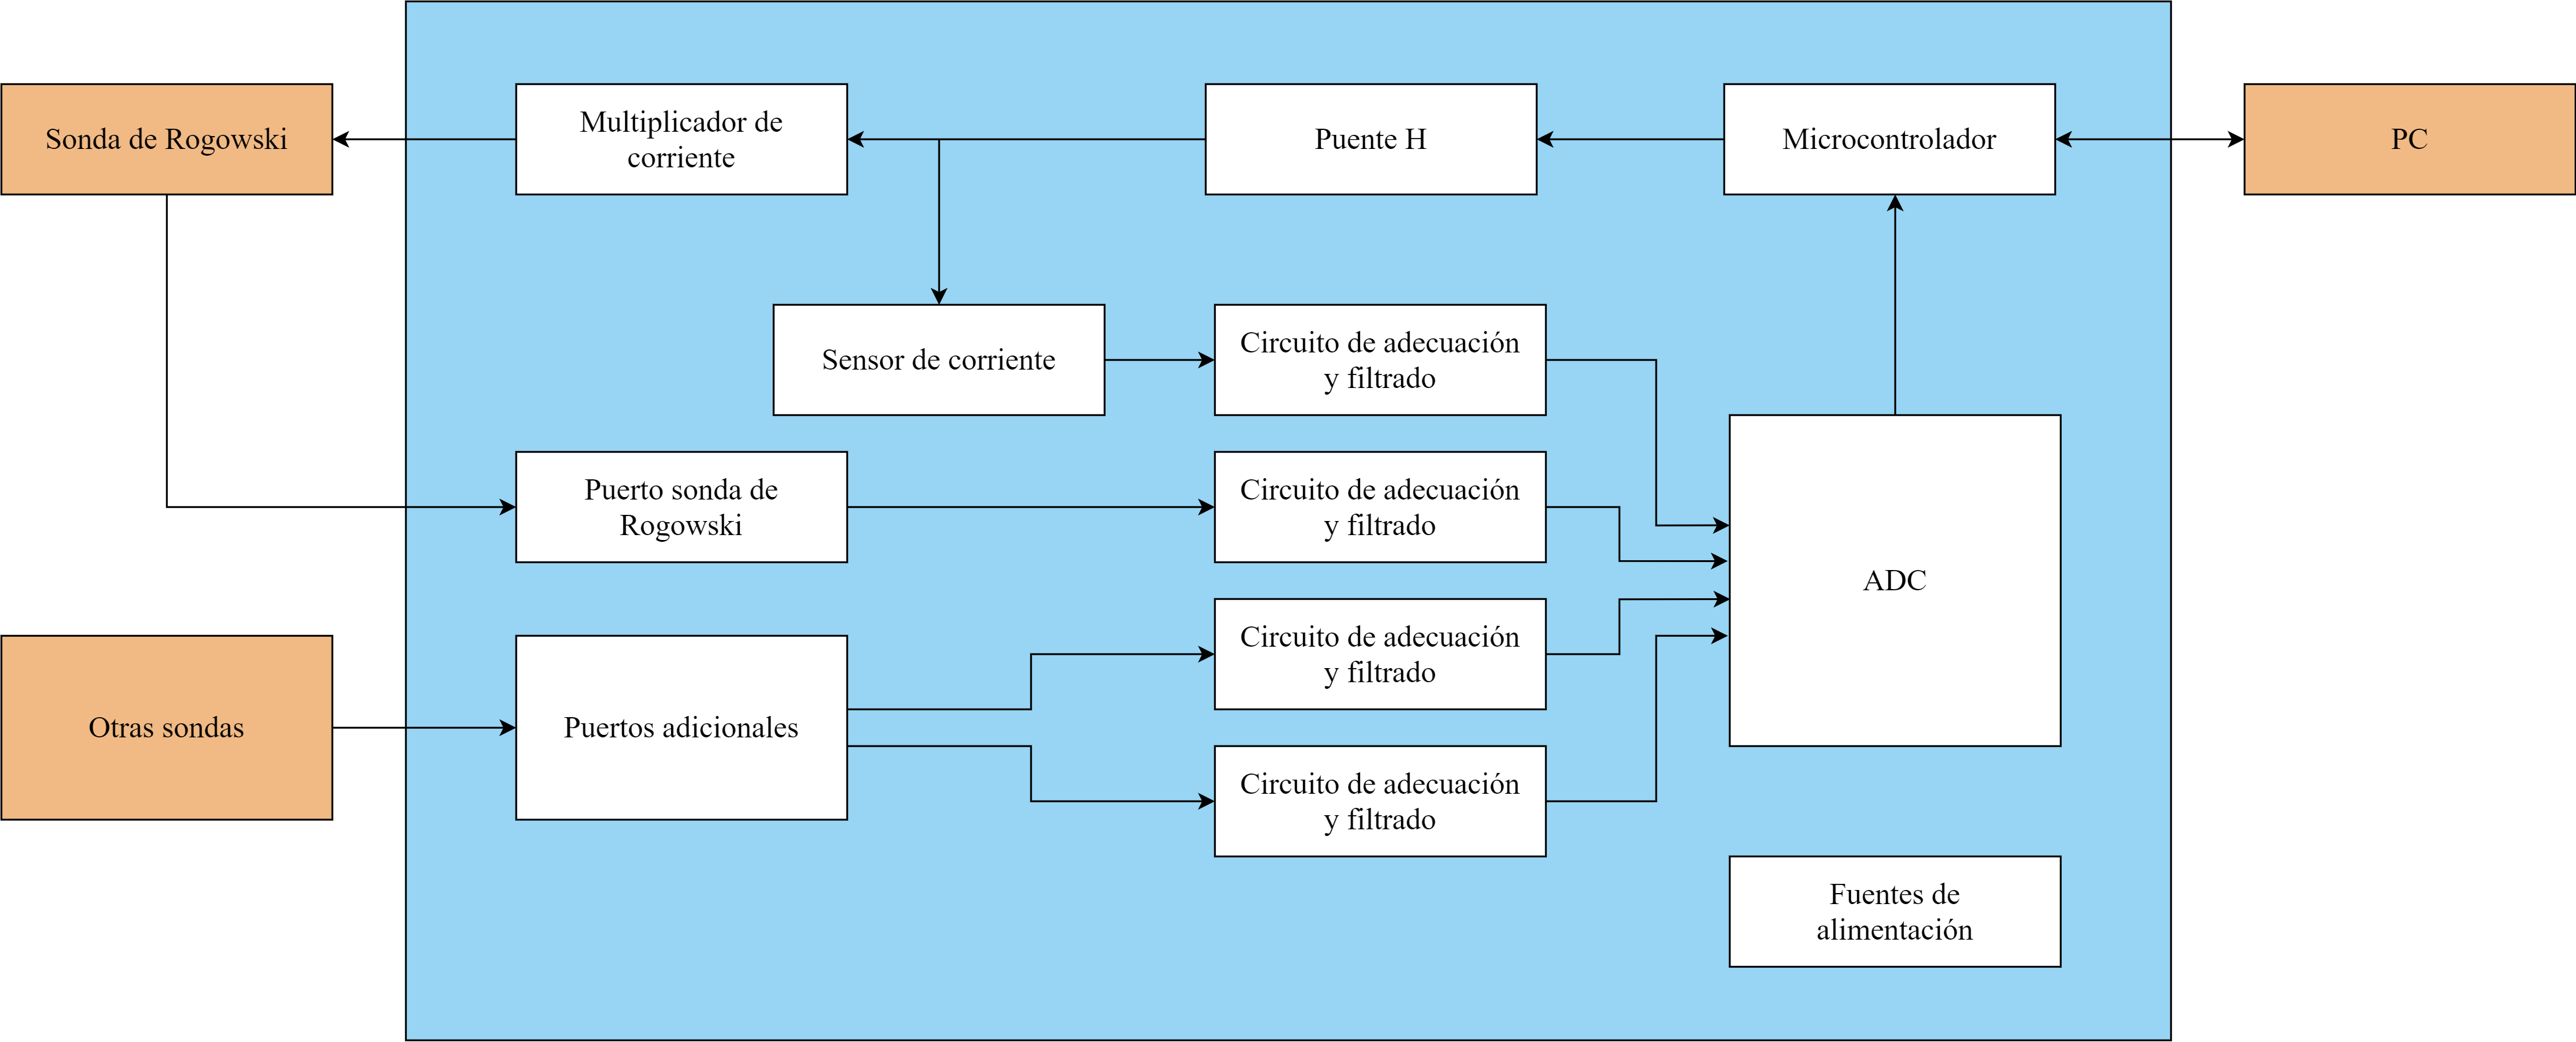
\includegraphics[width=\textwidth]{diagrams/bloques-general.png}
    \caption{Diagrama en bloques general del dispositivo}
    \label{fig:bloques-general}
  \end{figure}

Este instrumento permitirá generar corrientes que alimenten a las sondas a calibrar o caracterizar. Luego, las mediciones tomadas por estas sondas serán introducidas al instrumento para su posterior análisis.

Los resultados de estas calibraciones o caracterizaciones, serán mostradas a través de una interfaz gráfica en una PC, a la que estará conectado el instrumento. Esta permitirá controlar todas las funciones del mismo.


%% ----------------------------------------------------------------
\section{Diseño analógico y digital}
%% ----------------------------------------------------------------
\subfile{sections/analog-y-dig}

%% ----------------------------------------------------------------
\section{Diseño de firmware}
%% ----------------------------------------------------------------
\subfile{sections/firmware}

%% ----------------------------------------------------------------
\section{Diseño de software}
%% ----------------------------------------------------------------
\subfile{sections/software}


%% ----------------------------------------------------------------
\newpage
\printbibliography[heading=bibnumbered, title={Bibliografía}]
%% ----------------------------------------------------------------

%% ----------------------------------------------------------------
\newpage
\appendix
%% ----------------------------------------------------------------
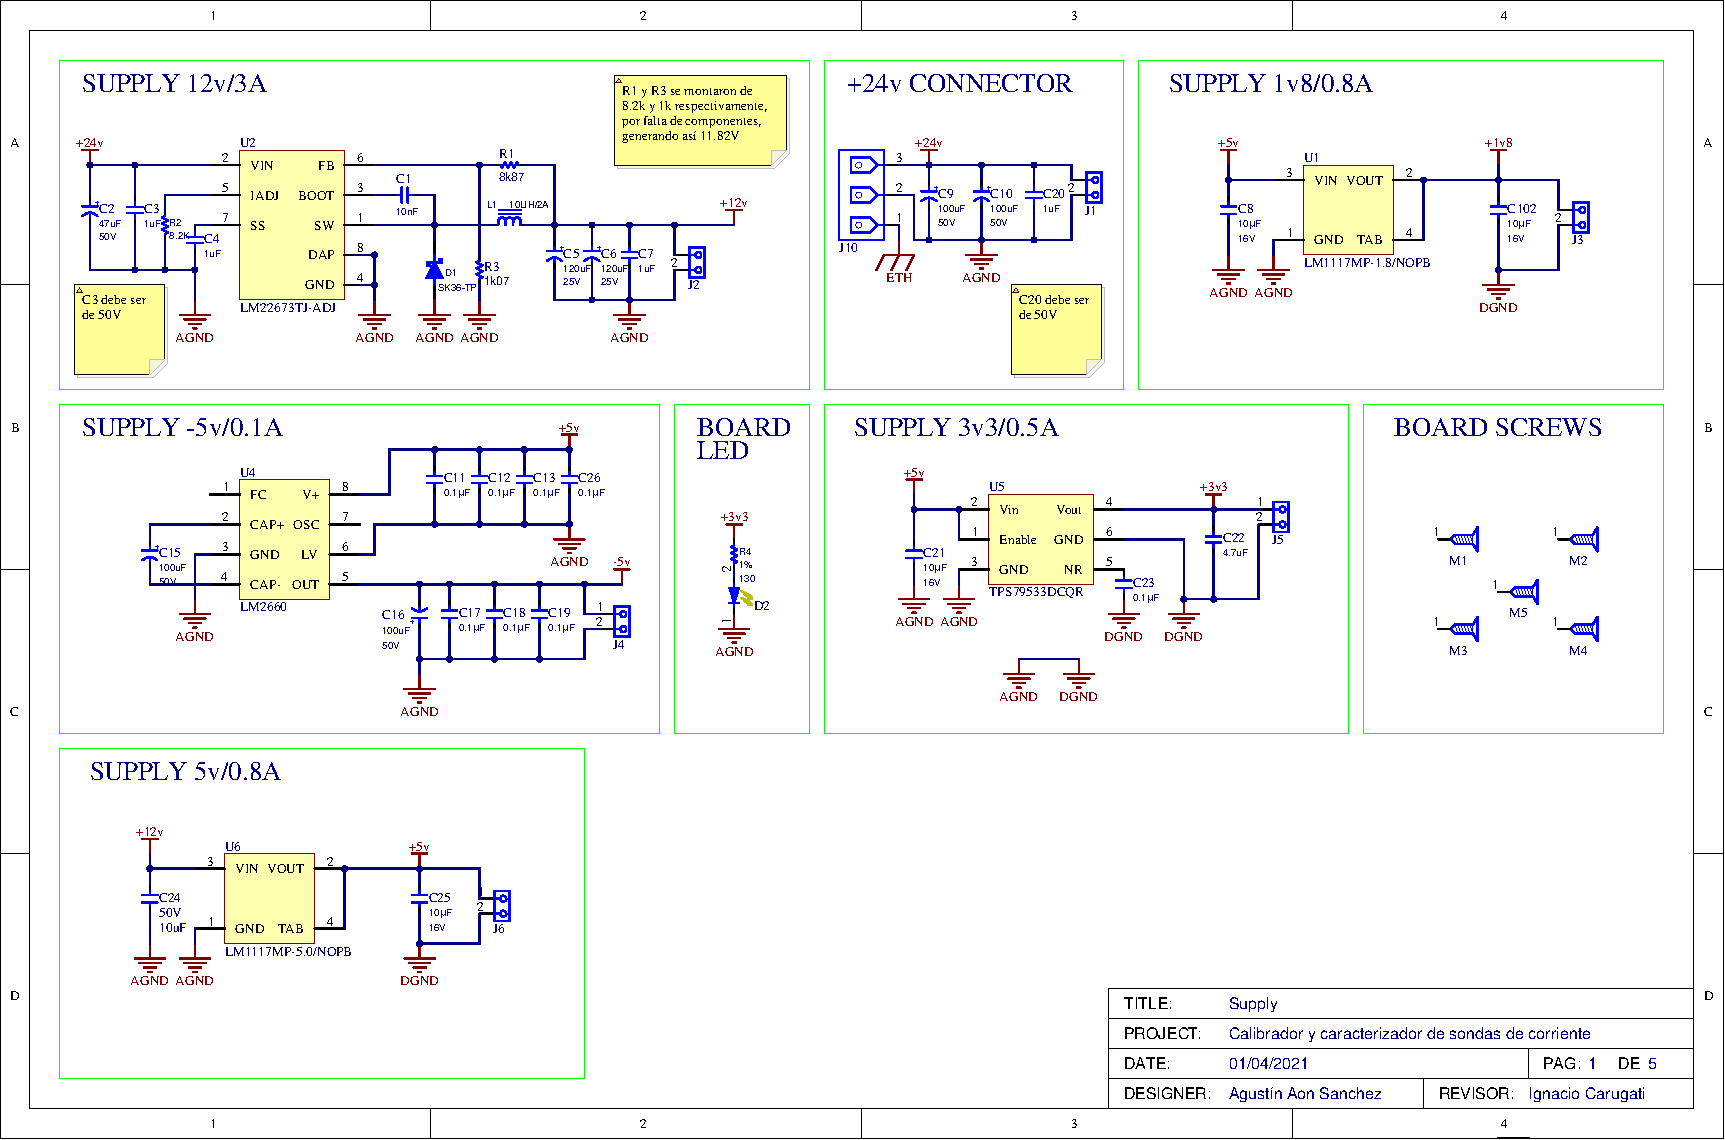
\includepdf[pages=1, angle=90, scale=0.7, pagecommand={\section{Esquemático completo}}]{../../hardware/Output/esquematico.pdf}

\includepdf[pages=2-, angle=90, scale=0.7, pagecommand={}]{../../hardware/Output/esquematico.pdf}


\end{document}
